
\documentclass[10pt]{article}
\linespread{1.25}

%%Make Parenthesis scale to fit whats inside
\newcommand{\parry}[1]{\left( #1 \right)}

%% Language and font encodings
\usepackage[english]{babel}
\usepackage[utf8x]{inputenc}
\usepackage[T1]{fontenc}
\usepackage{subcaption}
\usepackage[section]{placeins}

%% Sets page size and margins
\usepackage[a4paper,top=3cm,bottom=2cm,left=3cm,right=3cm,marginparwidth=1.75cm]{geometry}

%% No indents
\setlength\parindent{0pt}

%% Useful packages
\usepackage{amsmath}
\usepackage{amssymb}
\usepackage{amsfonts}
\usepackage{mathtools}
\usepackage{graphicx}
\usepackage{xcolor}
\usepackage[colorinlistoftodos]{todonotes}
\usepackage[colorlinks=true, allcolors=blue]{hyperref}
\usepackage{enumerate}
\usepackage{enumitem}
\usepackage[framed,autolinebreaks,useliterate]{mcode} %% MATLAB code
\usepackage{siunitx}
\usepackage{float}
\usepackage{scrextend}
\usepackage[final]{pdfpages}

%%Header & Footer
\usepackage[myheadings]{fullpage}
\usepackage{fancyhdr}
\usepackage{lastpage}
\usepackage{graphicx, wrapfig, subcaption, setspace, booktabs}

%% Define \therefore command
\def\therefore{\boldsymbol{\text{ }
\leavevmode
\lower0.4ex\hbox{$\cdot$}
\kern-.5em\raise0.7ex\hbox{$\cdot$}
\kern-0.55em\lower0.4ex\hbox{$\cdot$}
\thinspace\text{ }}}
\renewcommand{\vec}[1]{\boldsymbol{#1}}

%% Units
\DeclareSIUnit\year{yr}
\DeclareSIUnit\dollar{\$}
\DeclareSIUnit\celcius{C^{\circ}}
\DeclareSIUnit\mole{mole}
\def\conclusion{\quad \Rightarrow \quad}

\begin{document}


%----------------------------------------------------------------------------------------
%	TITLE PAGE
%----------------------------------------------------------------------------------------

%----------------------------------------------------------------------------------------
% HEADER AND FOOTER
%----------------------------------------------------------------------------------------
\pagestyle{fancy}
\fancyhf{}
\setlength\headheight{12pt}
\fancyhead[L]{\textbf{ES-APPM 447: Boundary Integral Methods}}
\fancyhead[R]{\textbf{HW 2 \qquad 5/21/2021 \qquad Liam O'Connor}}
\fancyfoot[R]{Page \thepage\ of \pageref{LastPage}}

\textit{I've copied the assignment below verbatim, it helps me keep track of things...}

\section*{Problem Statement}

Consider the singular Volterra integral equation
\begin{equation}
    x(s) = (1 + s)^{-1/2} + \frac{\pi}{8} - \frac{1}{4} \arcsin \Big( \frac{1 - s}{1 + s} \Big) - \frac{1}{4} \int_{0}^{s} \frac{x(t)}{(s - t)^{1/2}} dt. \label{main}
\end{equation}

The exact answer is $x_e(s) \equiv (1 + s)^{-1/2}$. Using a product integration analogue of the Trapezoid rule with constant step size $h$, solve the integral equation over the range $0 \leq s \leq 1$.

\section*{Quadrature Rule Derivation}
\subsection*{Instructions}
Determine a quadrature rule of the form
\begin{equation}
    \int_0^{s_i} (s_i - t)^{-1/2} x(t) dt = \sum_{j = 0}^i w_{ij} x(t_j)
\end{equation}

where $t_i = s_i$, $i = 0, \, ..., \, N$. The weights $w_{ij}$ are constructed by insisting that the rule be exact when $x(t)$ is a first degree polynomial. Identify the weights $w_{ij}$.

\subsection*{Solution}
With the given discretization, we begin by partitioning the integral into the sum of $N + 1$ integrals over sub-domains, i.e.

\begin{align*}
    \int_0^{s_i} (s_i - t)^{-1/2} x(t) dt &= \int_0^{h} \, (s_i - t)^{-1/2} x(t) \, dt + \int_h^{2h} \, (s_i - t)^{-1/2} x(t) \, dt + ... + \int_{(i - 1)h}^{ih} \, (s_i - t)^{-1/2} x(t) \, dt. 
    \intertext{Next we assume that $x(t)$ is given by a piece-wise linear, such that in each of the $N$ intervals evenly spaced by the set of points $x(ih)$, $x(t)$ is given by linear interpolation. This implies}
    &= \int_0^{h} \, (s_i - t)^{-1/2} \Big( x(0) +  \frac{(t-0)(x(h) - x(0))}{h} \Big) \, dt \\
    &\quad + \int_h^{2h} \, (s_i - t)^{-1/2} \Big( x(h) +  \frac{(t-h)(x(2h) - x(h))}{h} \Big) \, dt \\
    &\quad\quad \vdots \quad\quad\quad\quad\quad\quad\quad\quad\quad\quad\quad\quad \vdots \\
    &\quad + \int_{(i - 1)h}^{ih} \, (s_i - t)^{-1/2} \Big( x((i-1)h) +  \frac{(t - (i-1)h)(x(ih) - x((i-1)h))}{h} \Big) \, dt
\end{align*}
Collapsing into summation notation, we have that
\begin{align*}
    &= h^{-1}\sum_{j = 0}^{i-1} \int_{jh}^{(j+1)h} (s_i - t)^{-1/2} \Big( x(jh)h + (t-jh)(x((j+1)h) - x(jh)) \Big) \\
    &= h^{-1}\sum_{j = 0}^{i-1} \int_{jh}^{(j+1)h} (s_i - t)^{-1/2} \Bigg[x(jh)\Big( ((j+1)h - t)) \Big) + x((j+1)h)\Big( t - jh \Big)\Bigg]
    \intertext{We can shift the indices, yielding the weights}
    w_{ij} &= h^{-1}\begin{cases}
        \int_0^h (s_i - t)^{-1/2}(h - t) dt, \qquad j = 0 \\
        \int_{(j - 1)h}^{jh} (s_i - t)^{-1/2}(t - (j-1)h) dt + \int_{jh}^{(j+1)h} (s_i - t)^{-1/2}((j+1)h - t) dt, \qquad j = 1, \, 2, \, ..., \, i-1  \\
        \int_{(i-1)h}^{ih} (s_i - t)^{-1/2} (t - (i-1)h)dt, \qquad j = i
    \end{cases}
    \intertext{which satisfy the given criteria. The relevant indefinite integral is given by}
    &\quad\quad\quad\quad\quad\quad\quad\quad\quad\quad\quad\quad\int \frac{a + bt}{\sqrt{c + t}} dt = \frac{2}{3} \sqrt{c + t} \big( 3a + b(t - 2c) \big) + C
    \intertext{therefore}
    w_{ij} &= \begin{cases}
        \frac{2\sqrt{h}}{3} \big( (3 - 2i)\sqrt{i} + 2(i - 1)^{3/2} \big) , \qquad j = 0 \\
        \frac{2}{3} \sqrt{h}( 2(i - j + 1)^{3/2} - (2i - 2j + 3)\sqrt{i-j}) + \frac{2}{3}\sqrt{h} (2(i - j - 1)^{3/2} - (2i - 2j - 3)\sqrt{i - j}) \\
        \frac{2}{3} \sqrt{h} (h(i - 1) - h(i - 3)), \qquad j = i
    \end{cases}
    \intertext{simplifying gives}
    w_{ij} &= \sqrt{h}\begin{cases}
        \frac{2}{3} \big( (3 - 2i)\sqrt{i} + 2(i - 1)^{3/2} \big) , \hfill \qquad j = 0 \\
        \frac{4}{3}  \Big( (i - j + 1)^{3/2} - 2(i - j)^{3/2} + (i - j - 1)^{3/2} \Big), 
        \qquad j = 1,\,2,\,...,\, i-1\\
        \frac{4}{3}  , \qquad \hfill j = i
    \end{cases}
\end{align*}
With this in mind we continue with a more general discussion of how to solve the now-linear system and an analysis of the results.

\hspace{1cm}

\section*{Implementation}
\subsection*{Instructions}
Solve the singular integral equation numerically and determine the $N$ to give 6 decimal place accuracy. What is the observed order of convergence?
\clearpage
\subsection*{Solution}

We implement our discretization of (\ref{main}) by explicitly defining a vector $\vec{b}$ whose elements are given by
\begin{align*}
    b_i &= (1 + s_i)^{-1/2} + \frac{\pi}{8} - \frac{1}{4} \arcsin \Big( \frac{1 - s_i}{1 + s_i} \Big)
\end{align*}
Accordingly, we seek to obtain an approximate solution vector $\vec{sax}$ whose elements are satisfy $x_i \approx x(s_i)$. Lastly, we construct the matrix of weights $W$ whose elements are $1/4$ (the integral coefficient in (\ref{main})) the value of those derived in the last section. Notice that we only defined weights for $j \leq i$ Naturally we must ask: what are the remaining elements? 

Consider the first few elements of $\vec{x}$. For small $i$, the integral is only evaluated for/approximated by a few quadrature points. The remaining weights should be zero.

Therefore the discretized system is given by

\begin{align}
    \vec{x} &= \vec{b} - \frac{1}{4} \sum_{j = 0}^i w_{ij} x(t_j) \\
    &= \vec{b} - W \vec{x} \\
    &= (I + W)^{-1} \vec{b}
    \intertext{where $I$ is the identity matrix.}
\end{align}

Solving this system directly for large $N$ yields an approximation qualitatively indistinguishable from the analytical solution, is shown in Figure~\ref{fig:num1}.
Focusing on the error (since fortunately we are given the solution!), we obtain 6th decimal place accuracy at $N = 94$ as shown in Figure~\ref{fig:err}.
Plotting the error against resolution on a log-log scale, we obtain a slope of -2, indicating a power-law relationship  
\begin{equation*}
    ||\vec{x} - \vec{x_e}||_{\infty} \propto N^{-2}
\end{equation*}
with order of convergence 2. 
This is precisely what we expect for a trapezoidal method in a large $N$ and negligible floating-point error context.
Surprisingly, we obtain the theoretical result for very modest resolutions, indicating rapid convergence.


\begin{figure}[H]
    \centering
    \subfloat{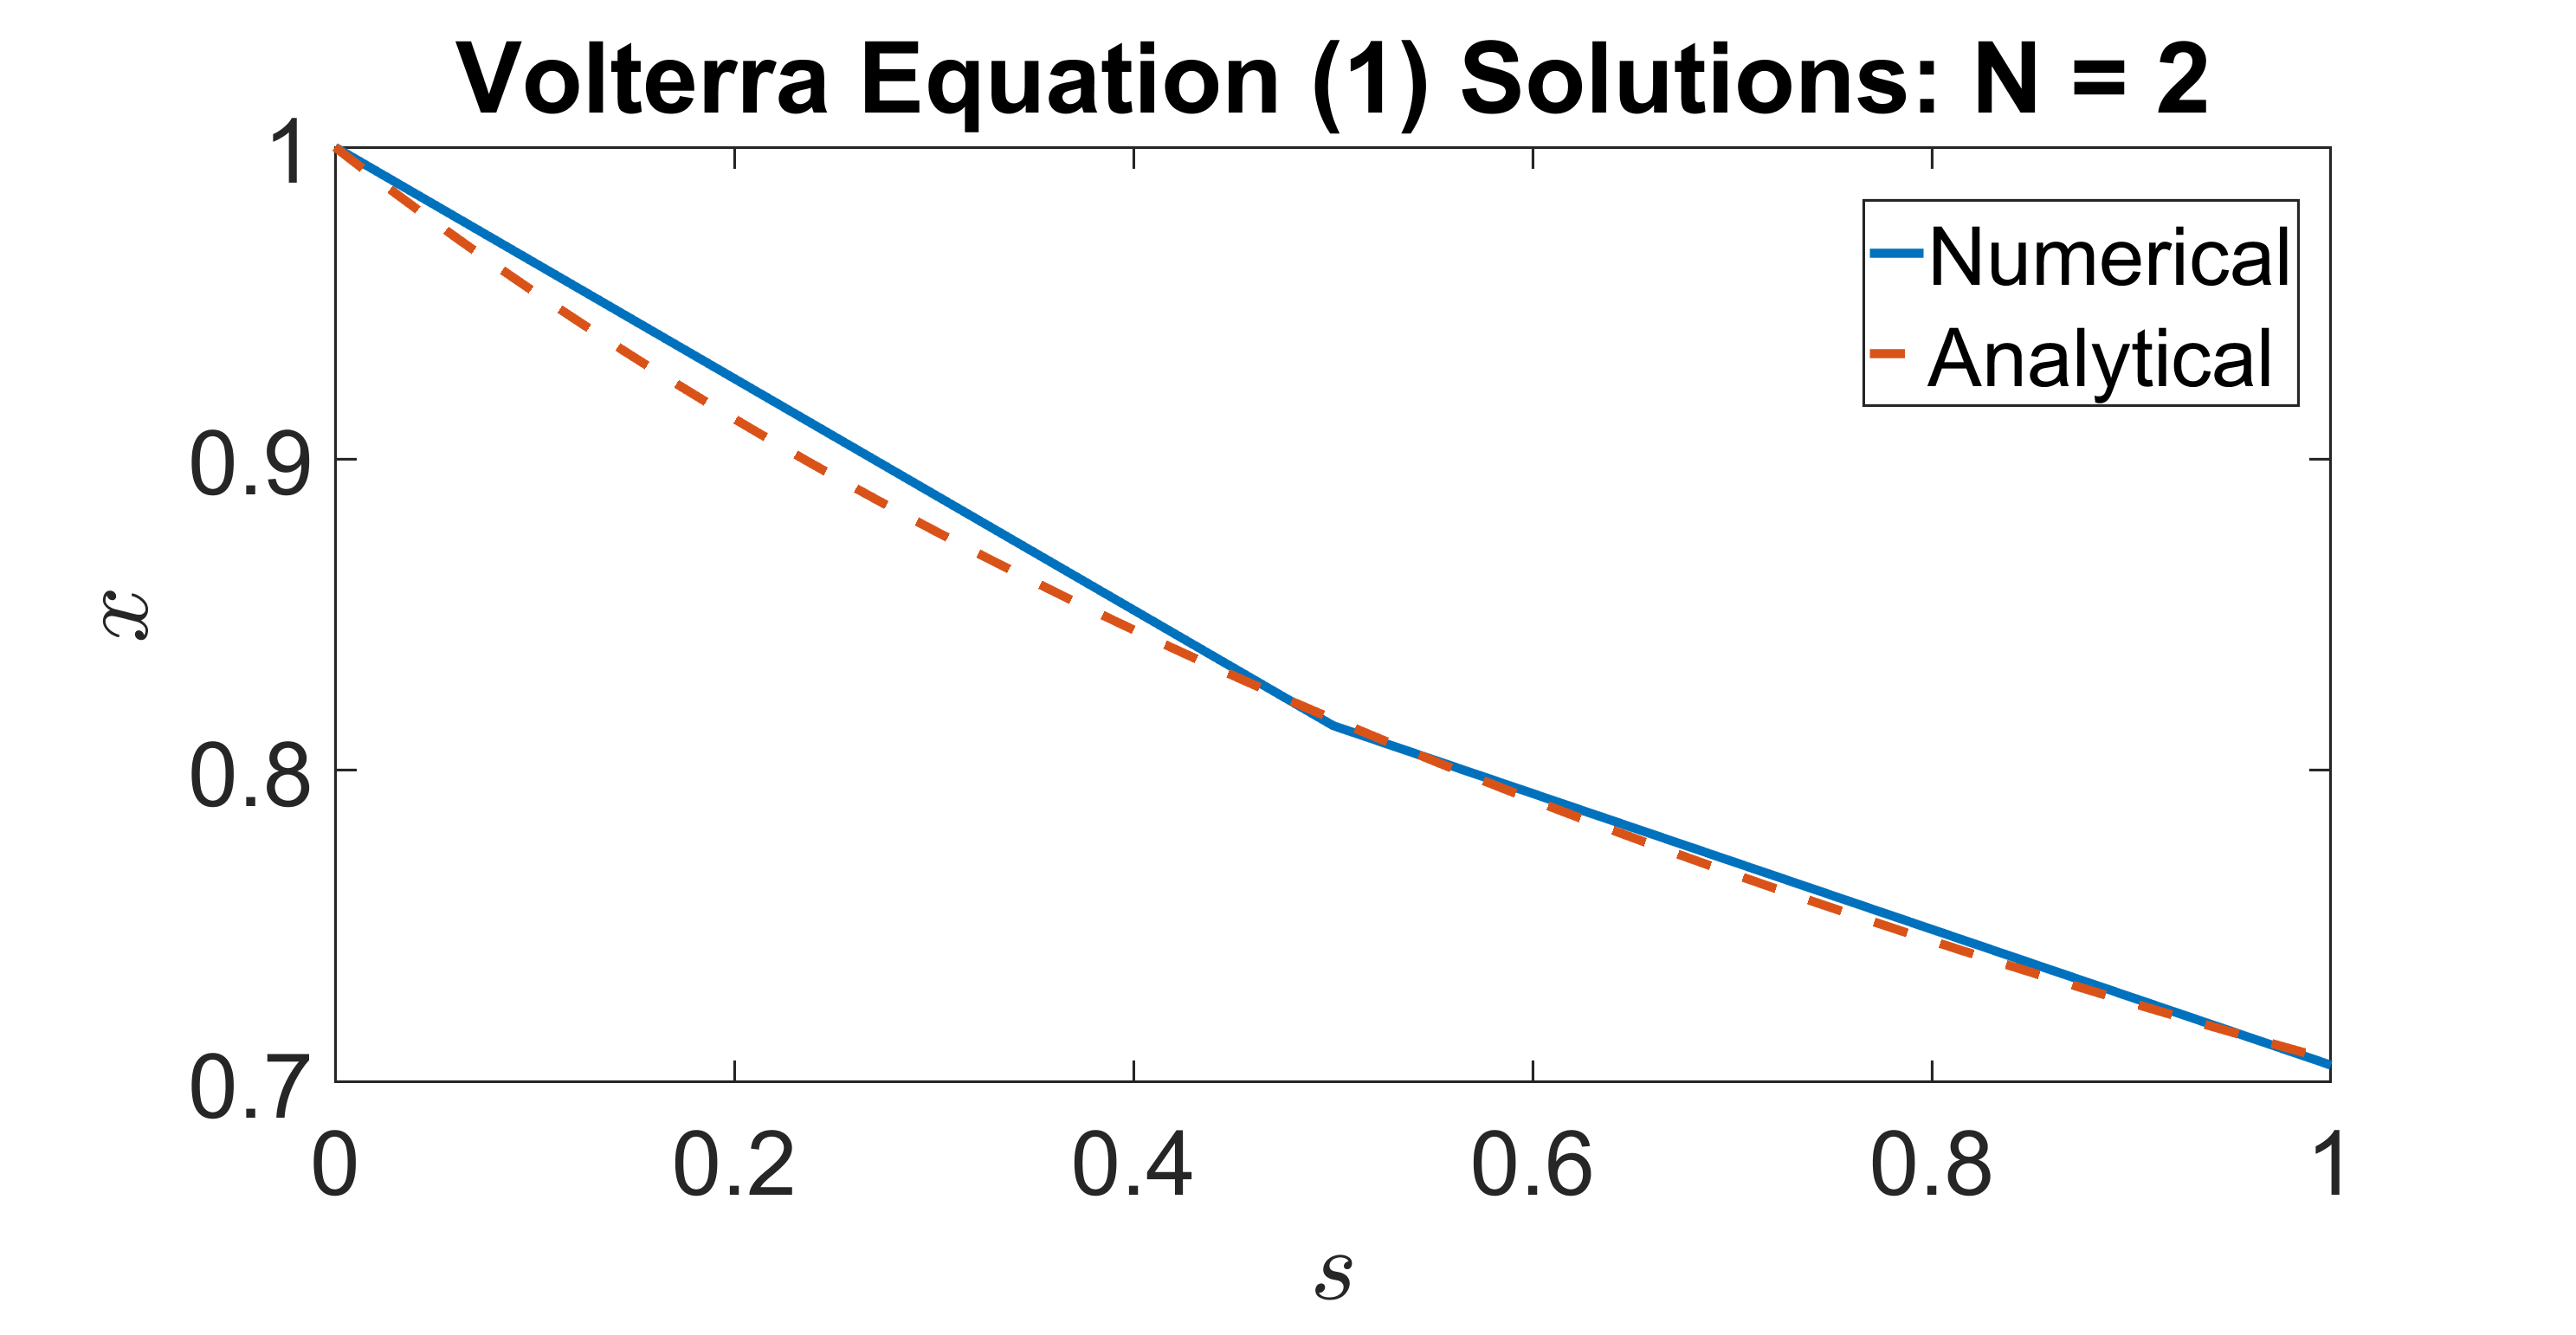
\includegraphics[width = 3.3in]{volt1.png}}
    \subfloat{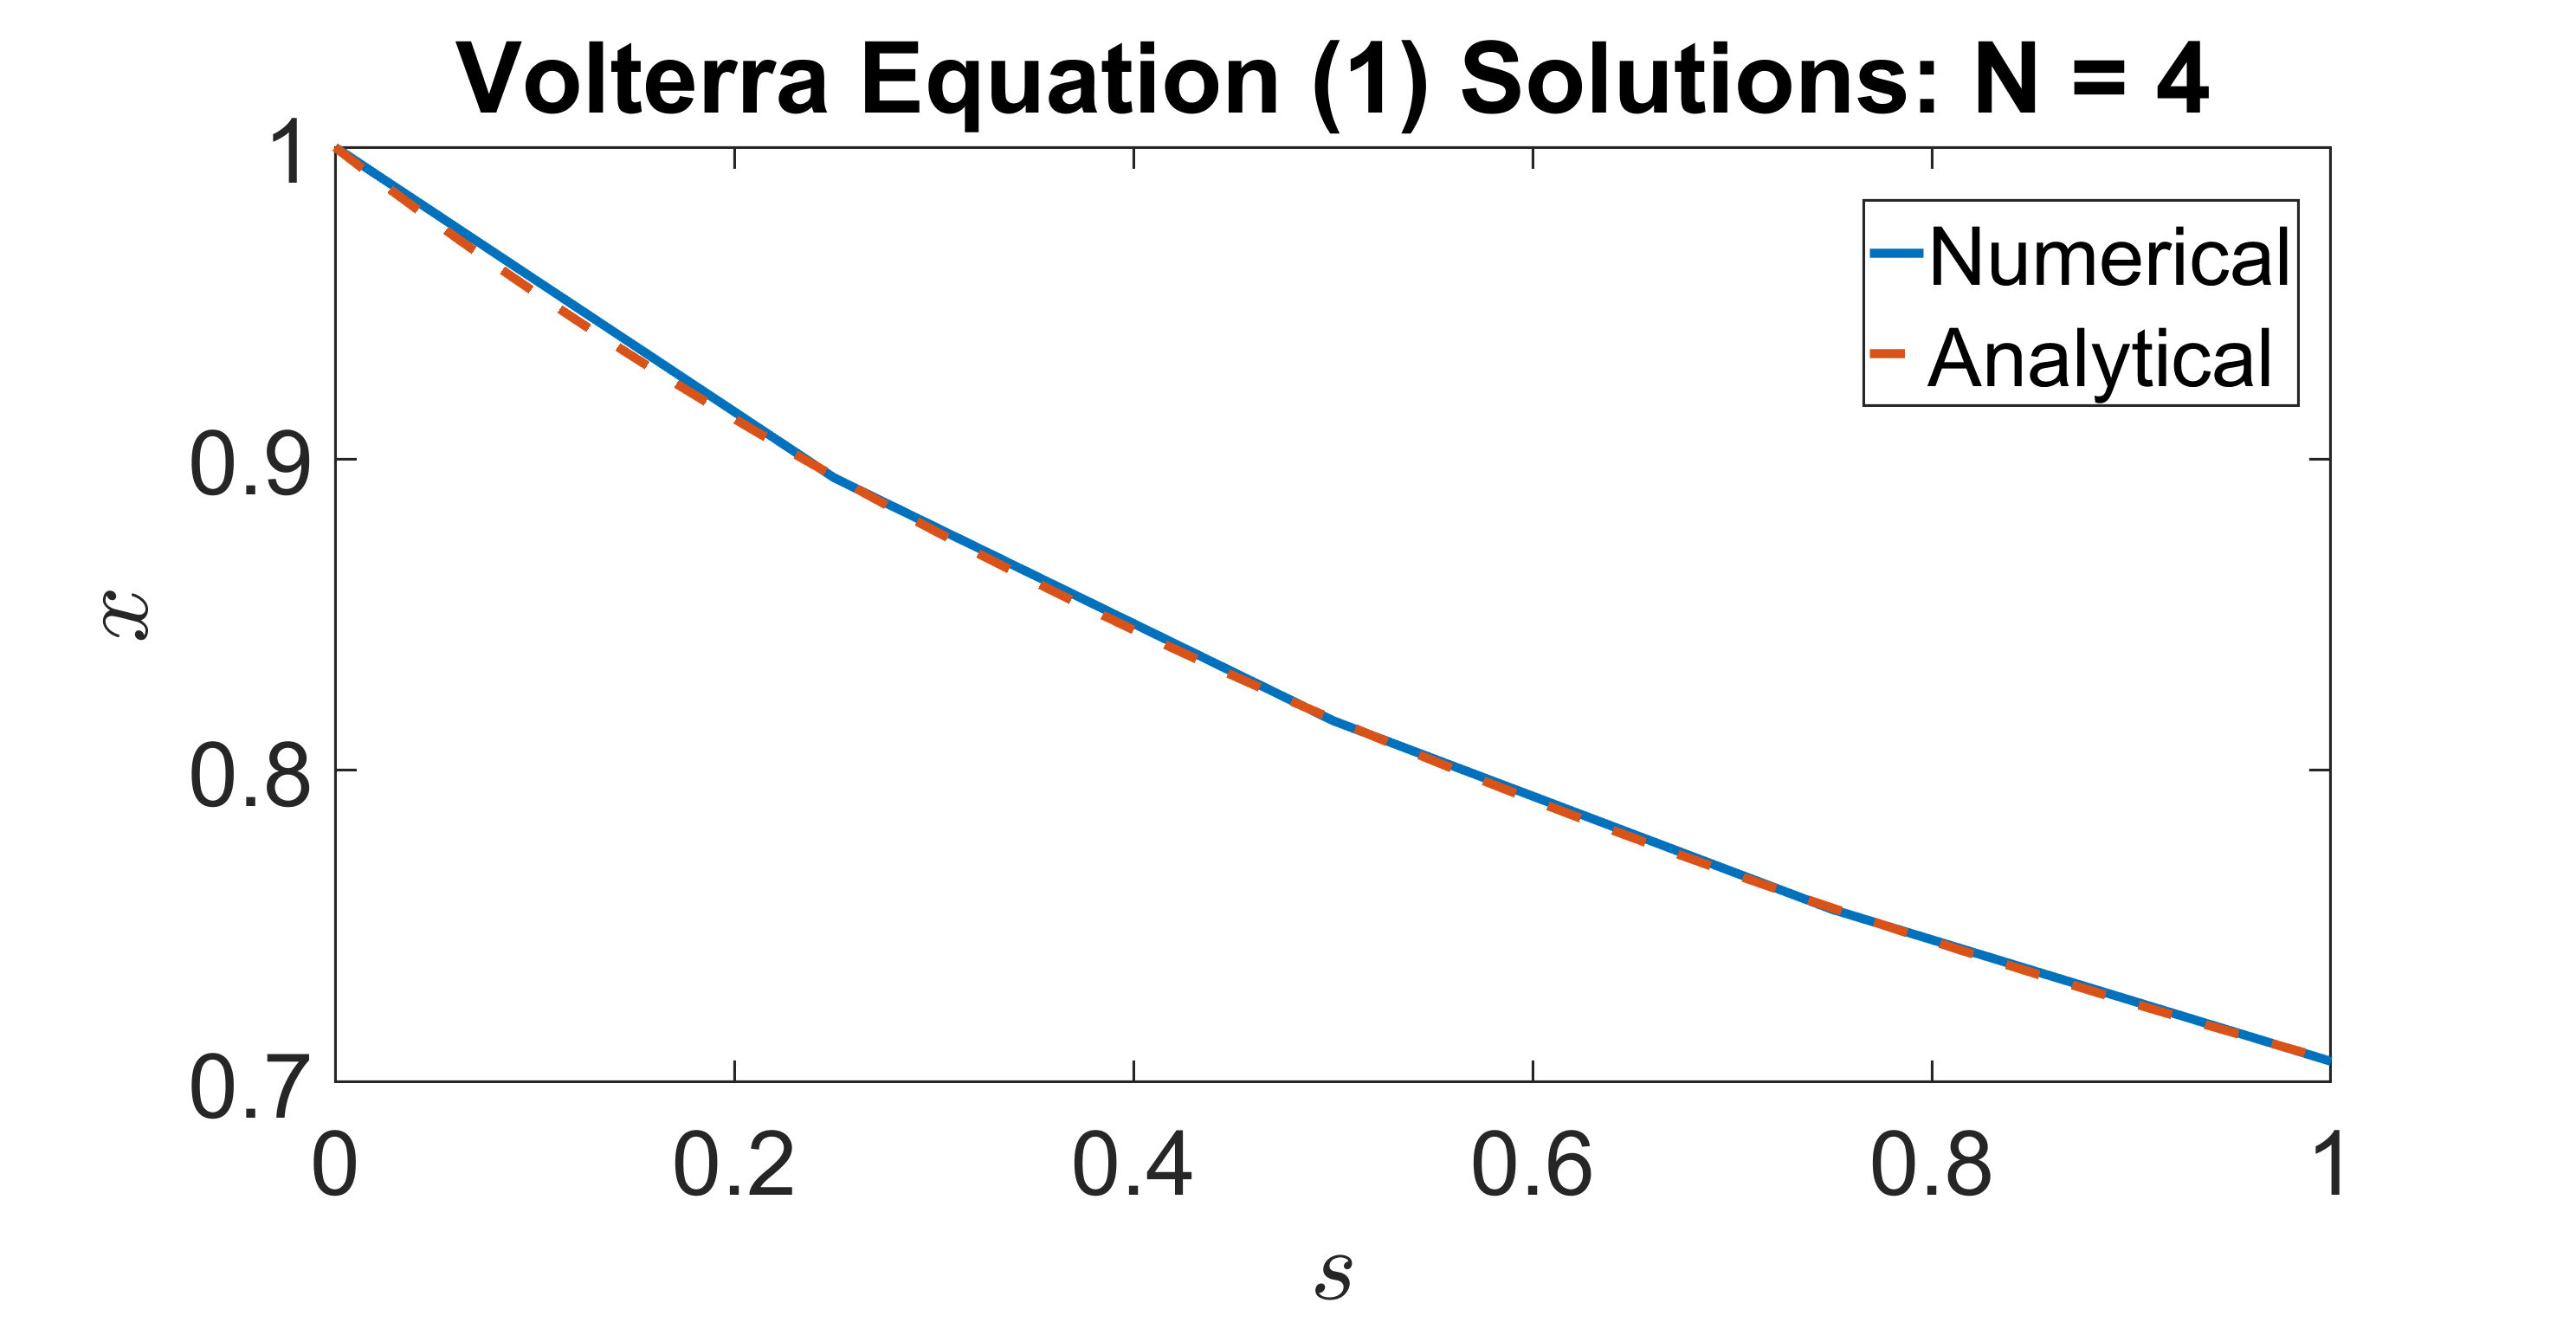
\includegraphics[width = 3.3in]{volt2.png}}
    \hfill
    \subfloat{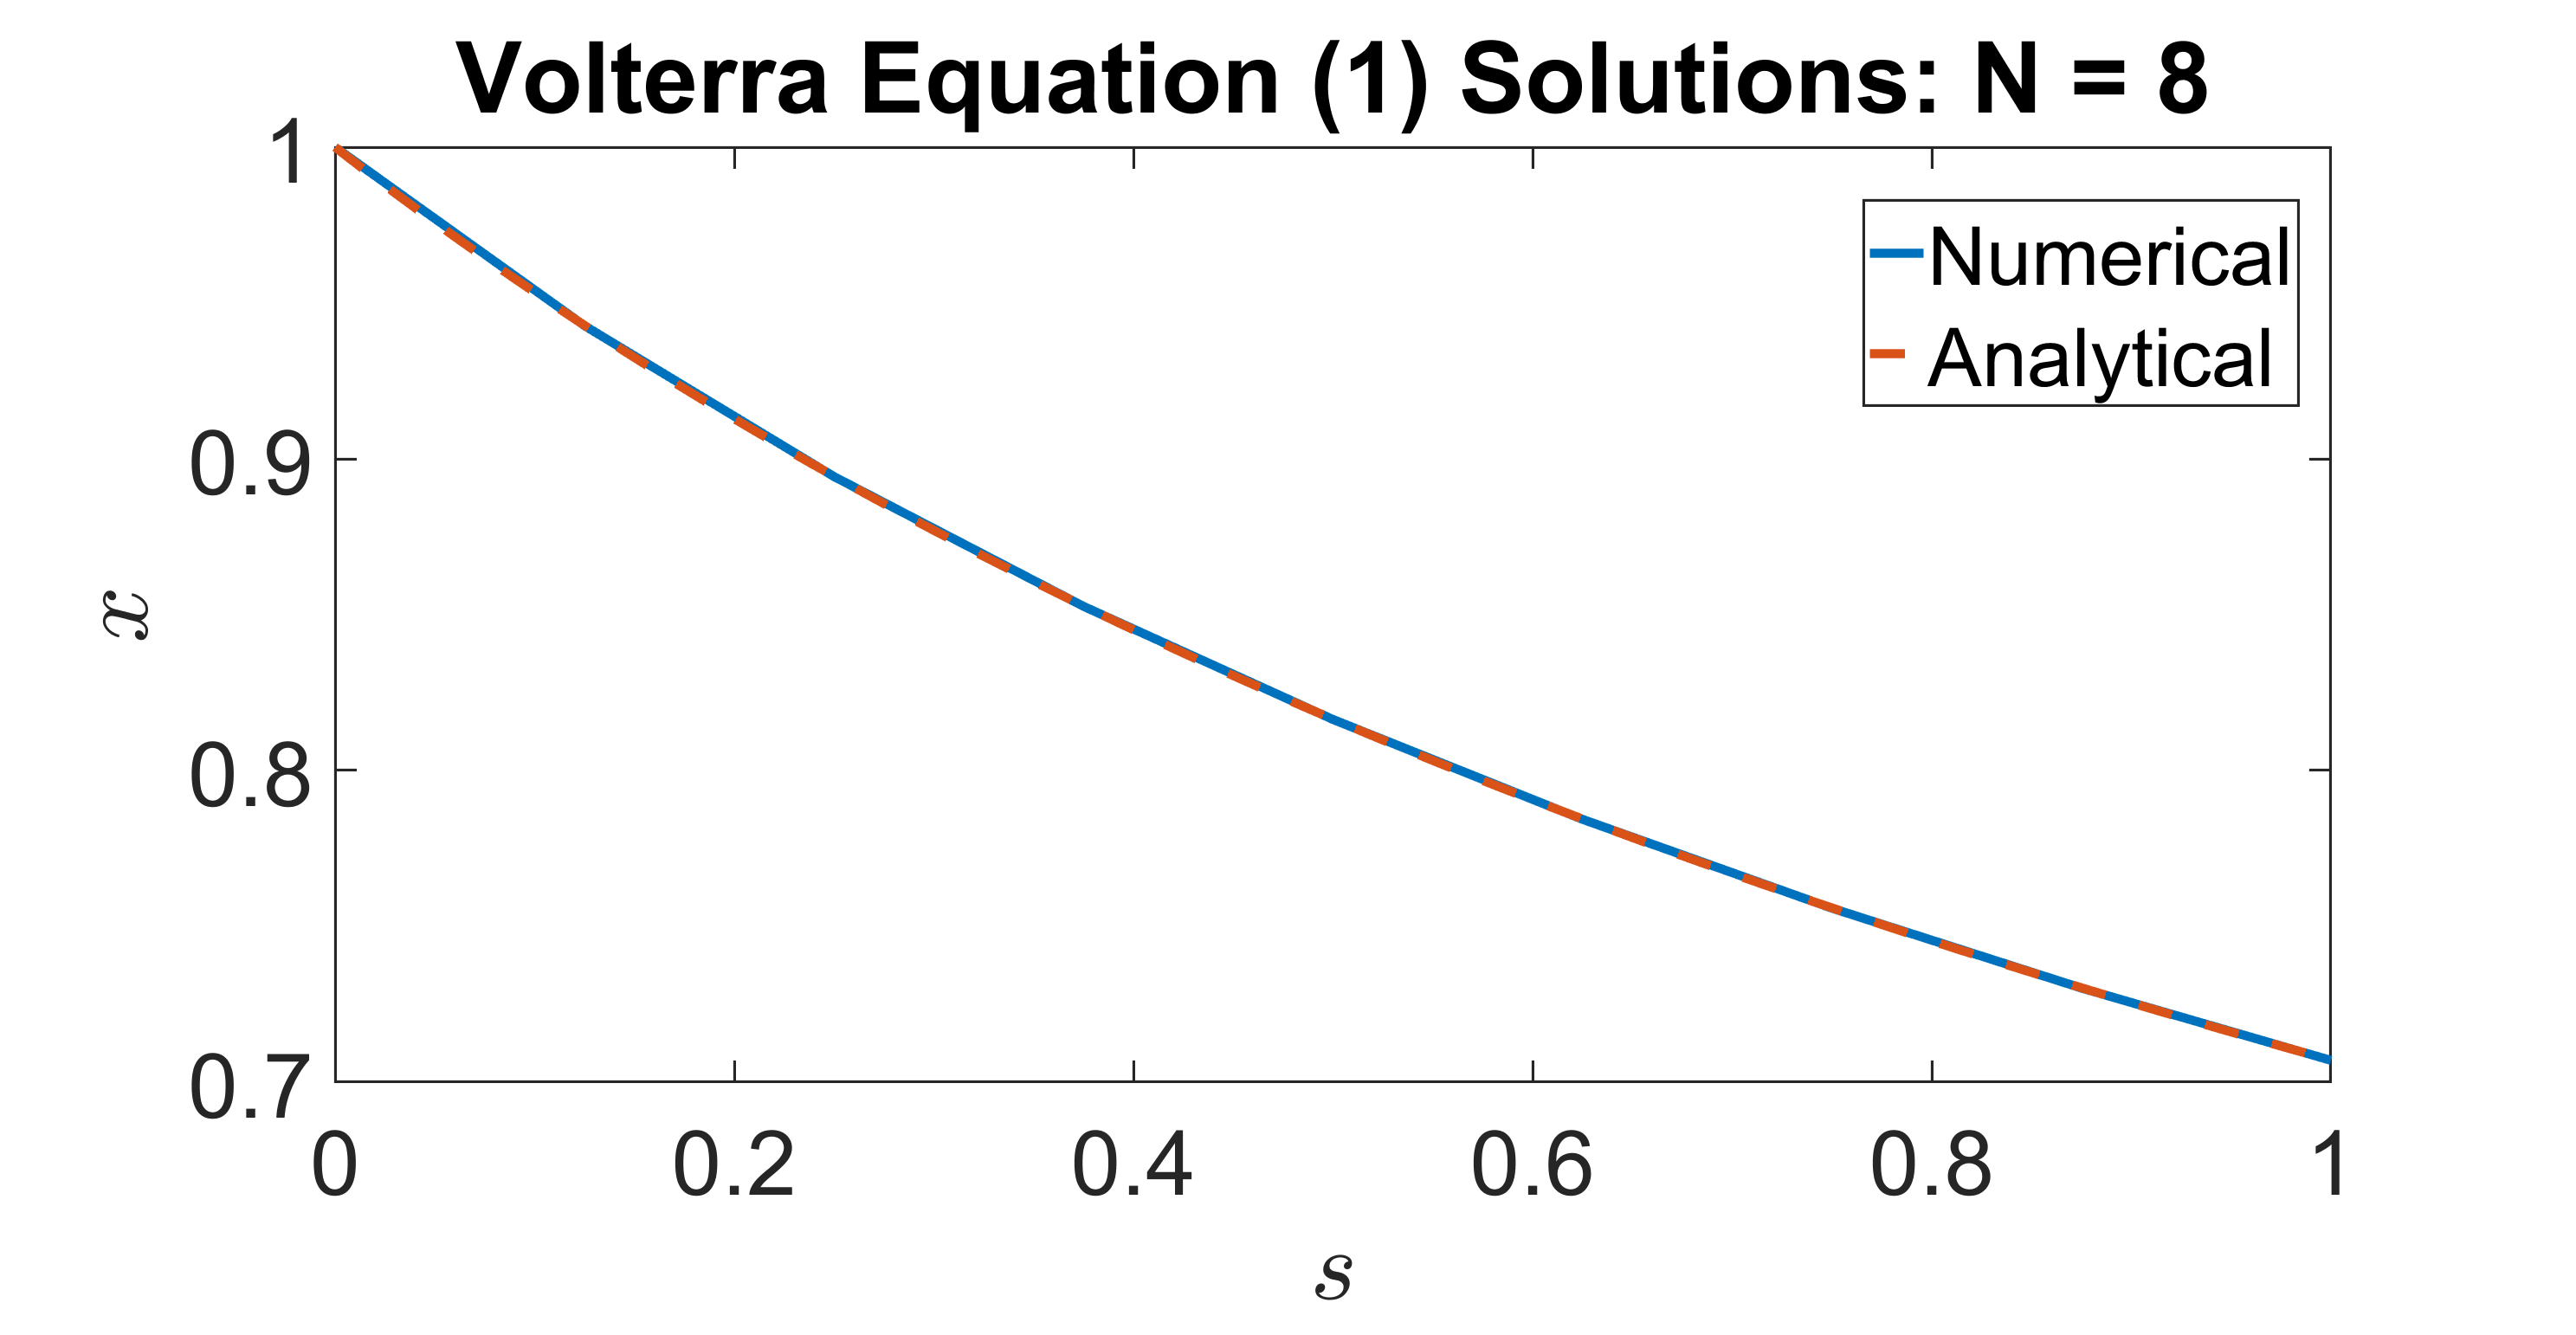
\includegraphics[width = 3.3in]{volt3.png}}
    \subfloat{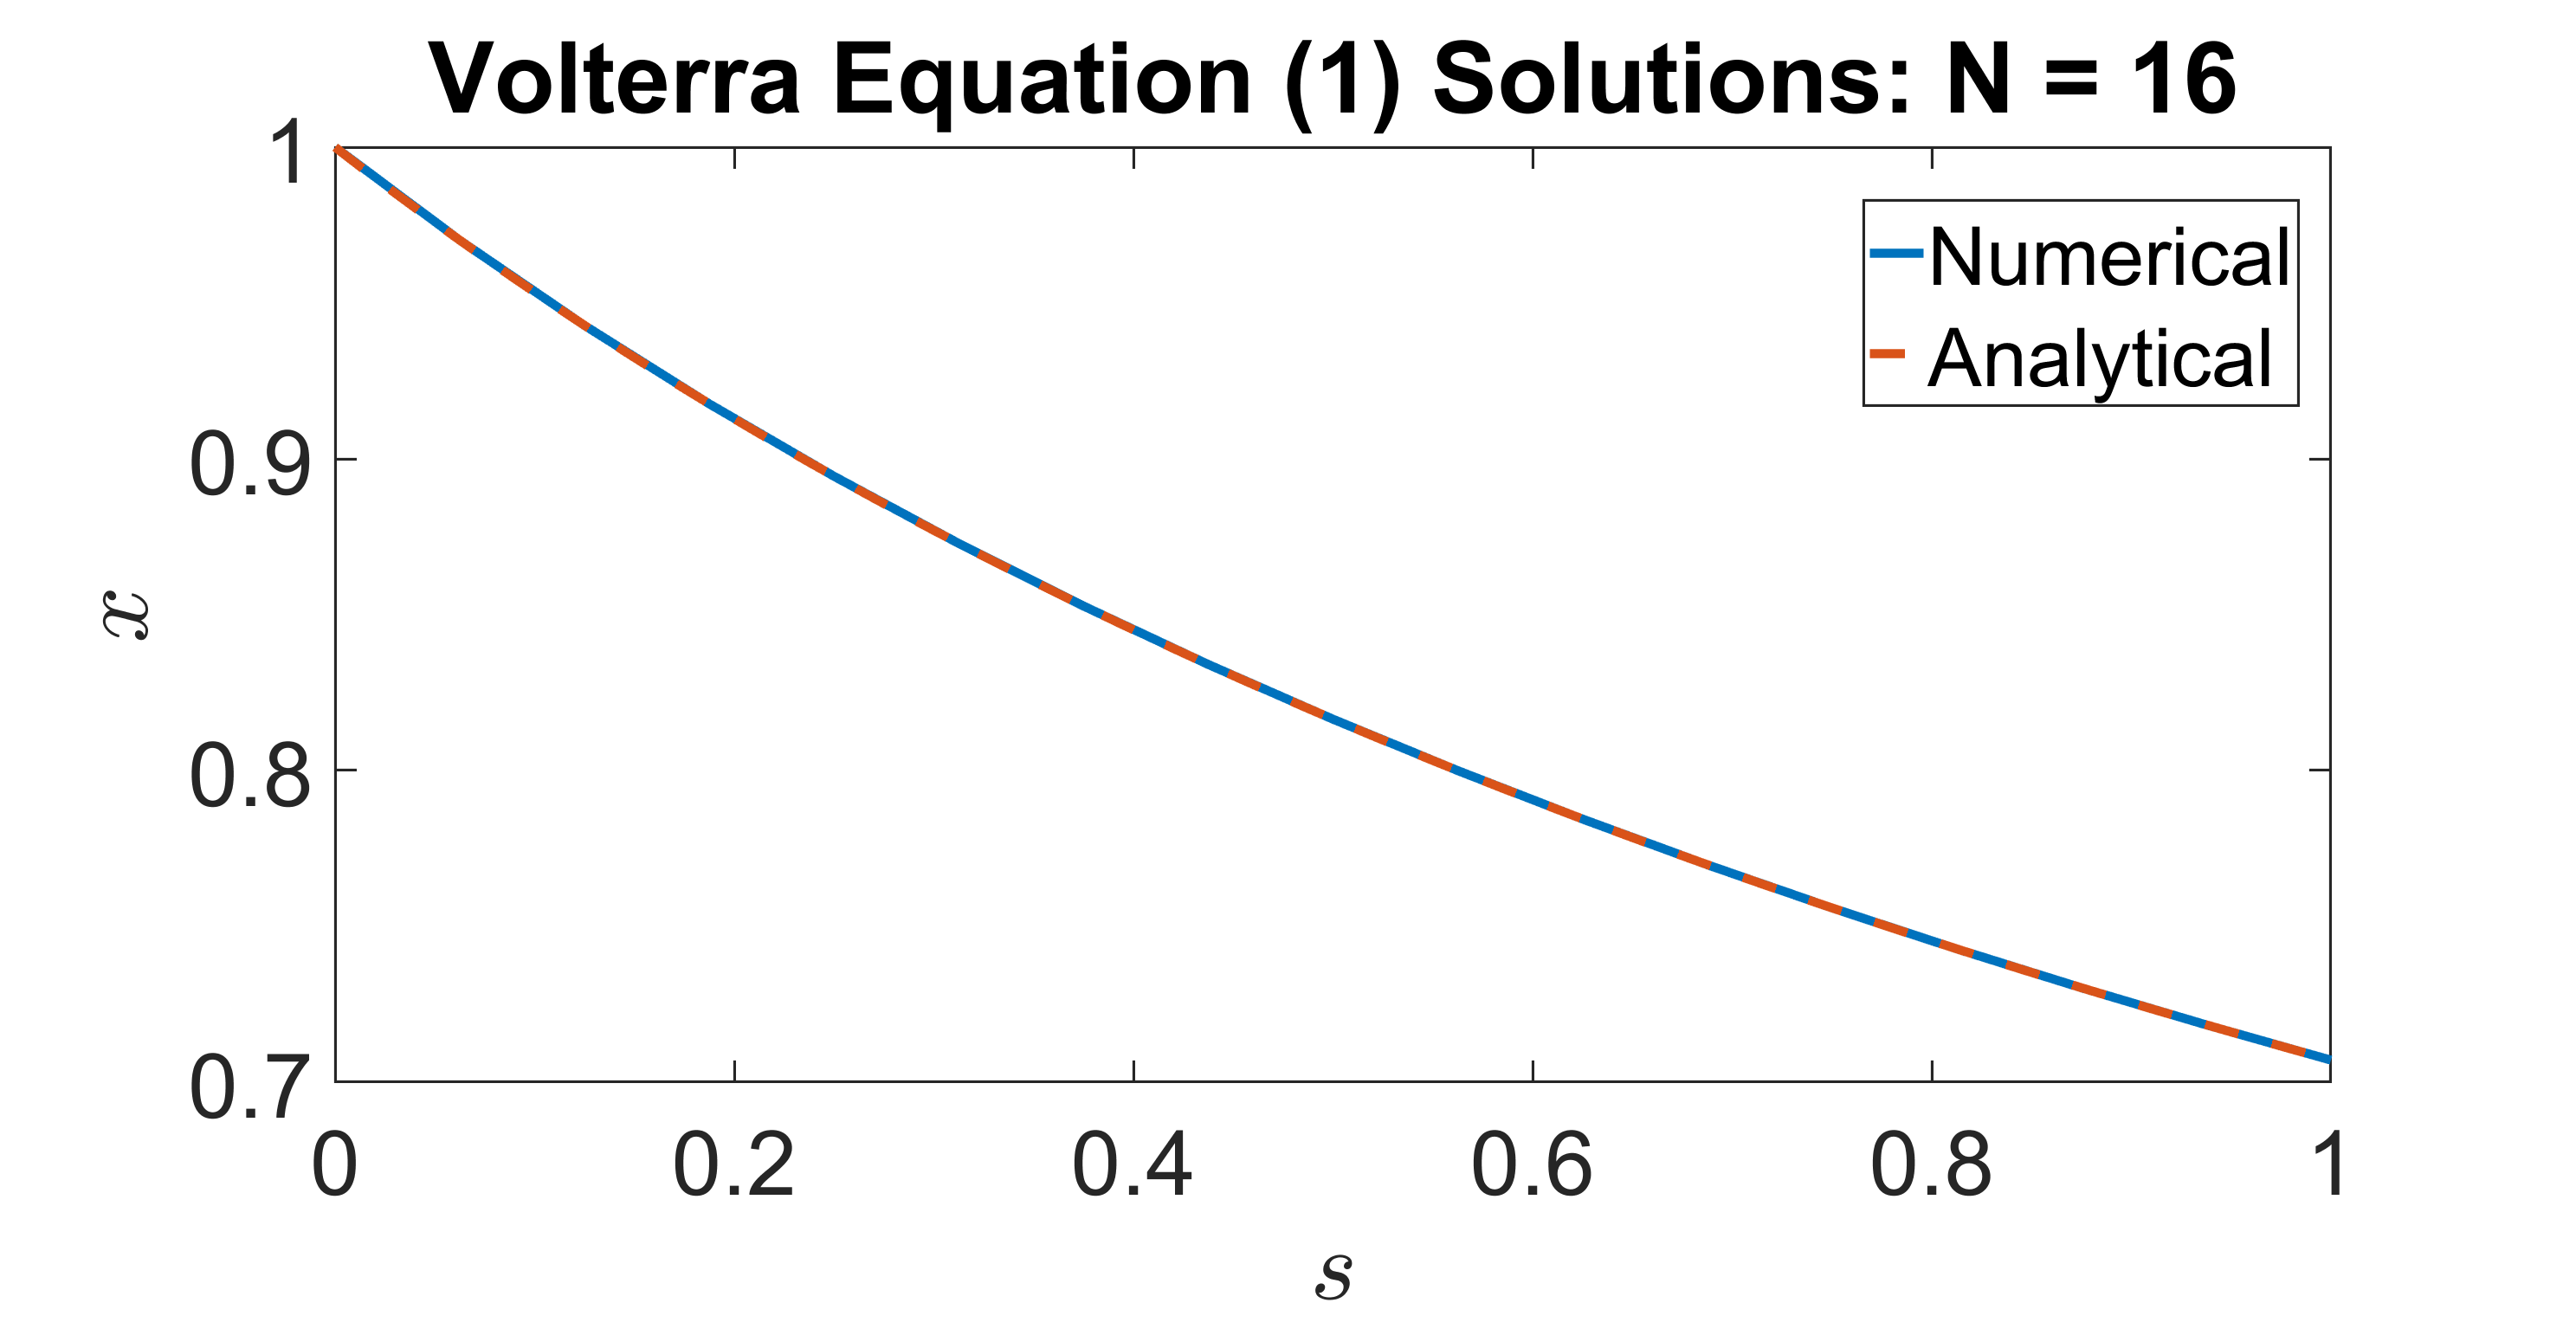
\includegraphics[width = 3.3in]{volt4.png}}
    \caption{Solutions to the Singular Volterra (\ref{main}): the numerical solution appears to converge to the analytical solution with increasing resolution $N$.}
    \label{fig:num1}
\end{figure}

\begin{figure}[H]
    \centering
    \subfloat{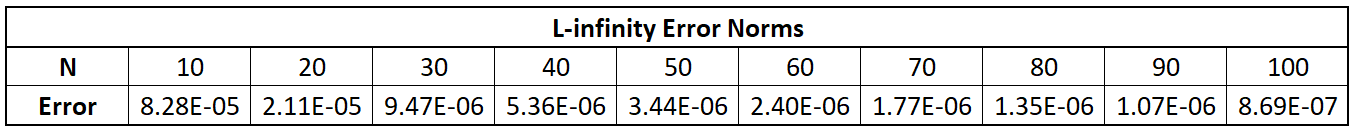
\includegraphics[width = 6.5in]{volt_er1.PNG}}
    \vspace{1cm}
    \subfloat{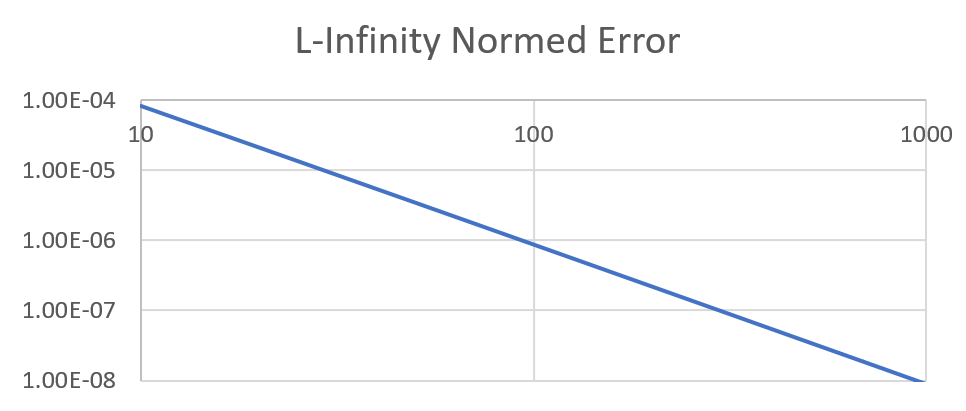
\includegraphics[width = 6.5in]{volt_er2.PNG}}
    \caption{$L-\infty$ errors are given for modest resolutions.}
    \label{fig:err}
\end{figure}

\begin{lstlisting}
    %%%%%%%%%%%%%%%%%%%%%%%%%%%%%%%%%%%%%
    % Solves the Singular Volterra Integral Equation:
    % $x(s) = (1 + s)^{-1/2} + \frac{\pi}{8} - \frac{1}{4}\arcsin \Big( \frac{1 - s}{1 + s} \Big) 
    %  - \frac{1}{4} \int_{0}^{s} \frac{x(t)}{(s - t)^{1/2}} dt$ on $0 < s < 1$
    %   via Trapezoidal product integration
    %%%%%%%%%%%%%%%%%%%%%%%%%%%%%%%%%%%%%
    
    % Parameters
    N_vec = [90:1:100];
    
    for N = N_vec
        % Allocation
        s = linspace(0, 1, N + 1)';
        b = 1 ./ sqrt(1 + s) + pi / 8 - asin((1 - s) ./ (1 + s)) / 4;
        W = zeros(N + 1, N + 1);
        xe = 1 ./ sqrt(s + 1);
    
        % We let the first row have zero weights because this is associated with  
        % s = 0. The contribution of the integral term is zero here so the weight
        % shall be as well.
        for row = 2:N + 1 %i
            for col = 1:row %j
                if col == 1
                    W(row, col) = (row - 2)^(3/2) - sqrt(row - 1) * (2 * (row - 1) - 3)/2;
                elseif col == row
                    W(row, col) = 1;
                else
                    W(row, col) = (row - col + 1)^(3/2) - 2 * (row - col)^(3/2) + (row - col - 1)^(3/2);
                end
            end
        end
        
        x = linsolve(eye(N + 1) + W / sqrt(N)/3,  b);
    %     disp(strcat("N = ", num2str(N), ": error = ", num2str(norm(x - xe, inf))))
        disp(num2str(norm(x - xe, inf)))
        
    end
\end{lstlisting}

\end{document}
